\section{MomeaProbe/MomeaCapture: Captura continua de dados}

No escopo do Projeto \textbf{MOMEA — Monitoramento Online de Rotores de Turbinas pelo Método de Emissão Acústica}, desenvolvido pelo grupo de pesquisa da Itaipu ParqueTec em parceria com a Itaipu Binacional, foram implementadas aplicações experimentais voltadas à análise de sinais acústicos e vibromecânicos obtidos de motobombas submetidas a diferentes condições de operação.  

O sistema \textbf{MomeaProbe/MomeaCapture} atua como plataforma de aquisição de dados, realizando a captura simultânea de sinais de Emissão Acústica (EA), vibração e/ou pressão em alta taxa de amostragem. O MomeaProbe é o hardware composto por dois ADCs de 12 bits operando a 8Msps e transmissão via interface USB~3.0, a placa e como mostrada na Figura ~\ref{fig:MomeaProbe12USB}.

\begin{figure}[H]
    \centering
    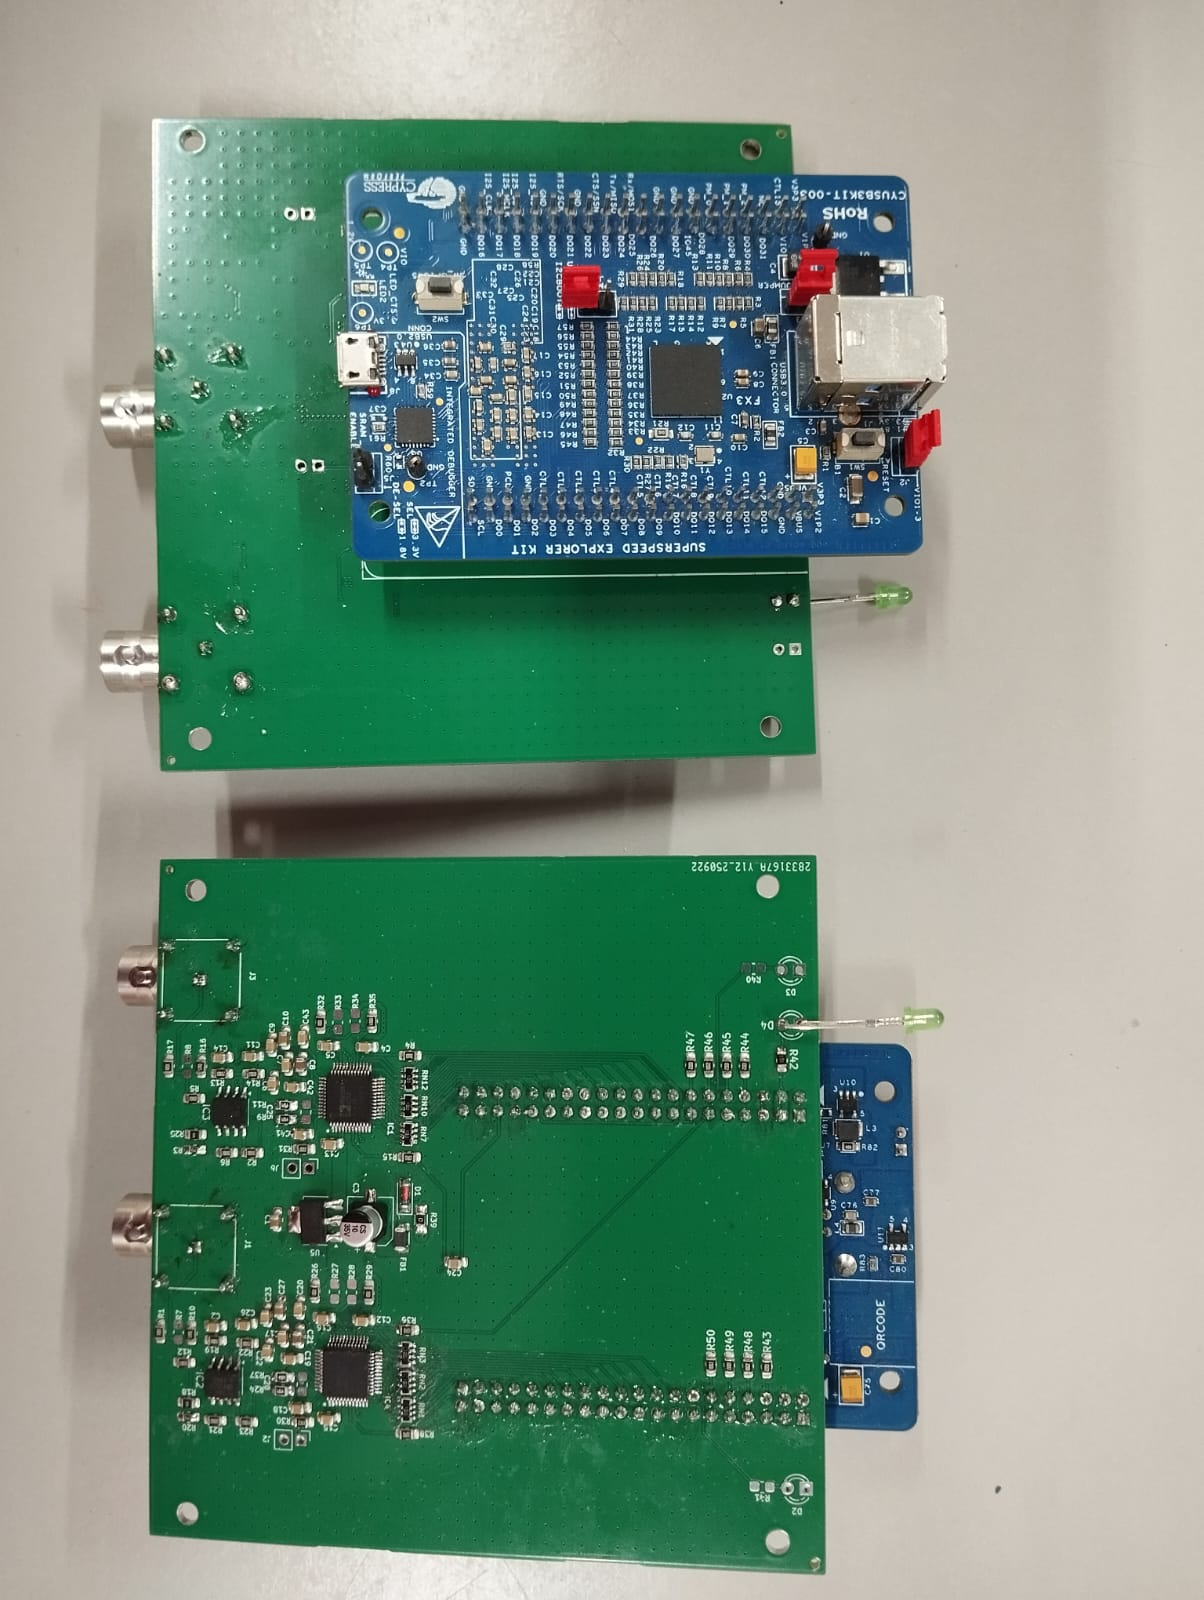
\includegraphics[width=0.5\linewidth, angle=90]{figs/PlacasADC_AD9226.jpeg}
    \caption{Placas de captura de sinais MomeaProbe12USB}
    \label{fig:MomeaProbe12USB}
\end{figure}

Os dados adquiridos no ambiente \textbf{MomeaCapture}, Figura ~\ref{fig:MomeaCapture}, uma aplicação desenvolvida em C++/Qt, responsável pelo gerenciamento da transferência, compressão, armazenamento e visualização dos sinais. Essa arquitetura possibilita o registro contínuo de longas séries temporais com resolução temporal suficiente para a análise espectral de fenômenos de cavitação e microfalhas estruturais.

\begin{figure}[H]
    \centering
    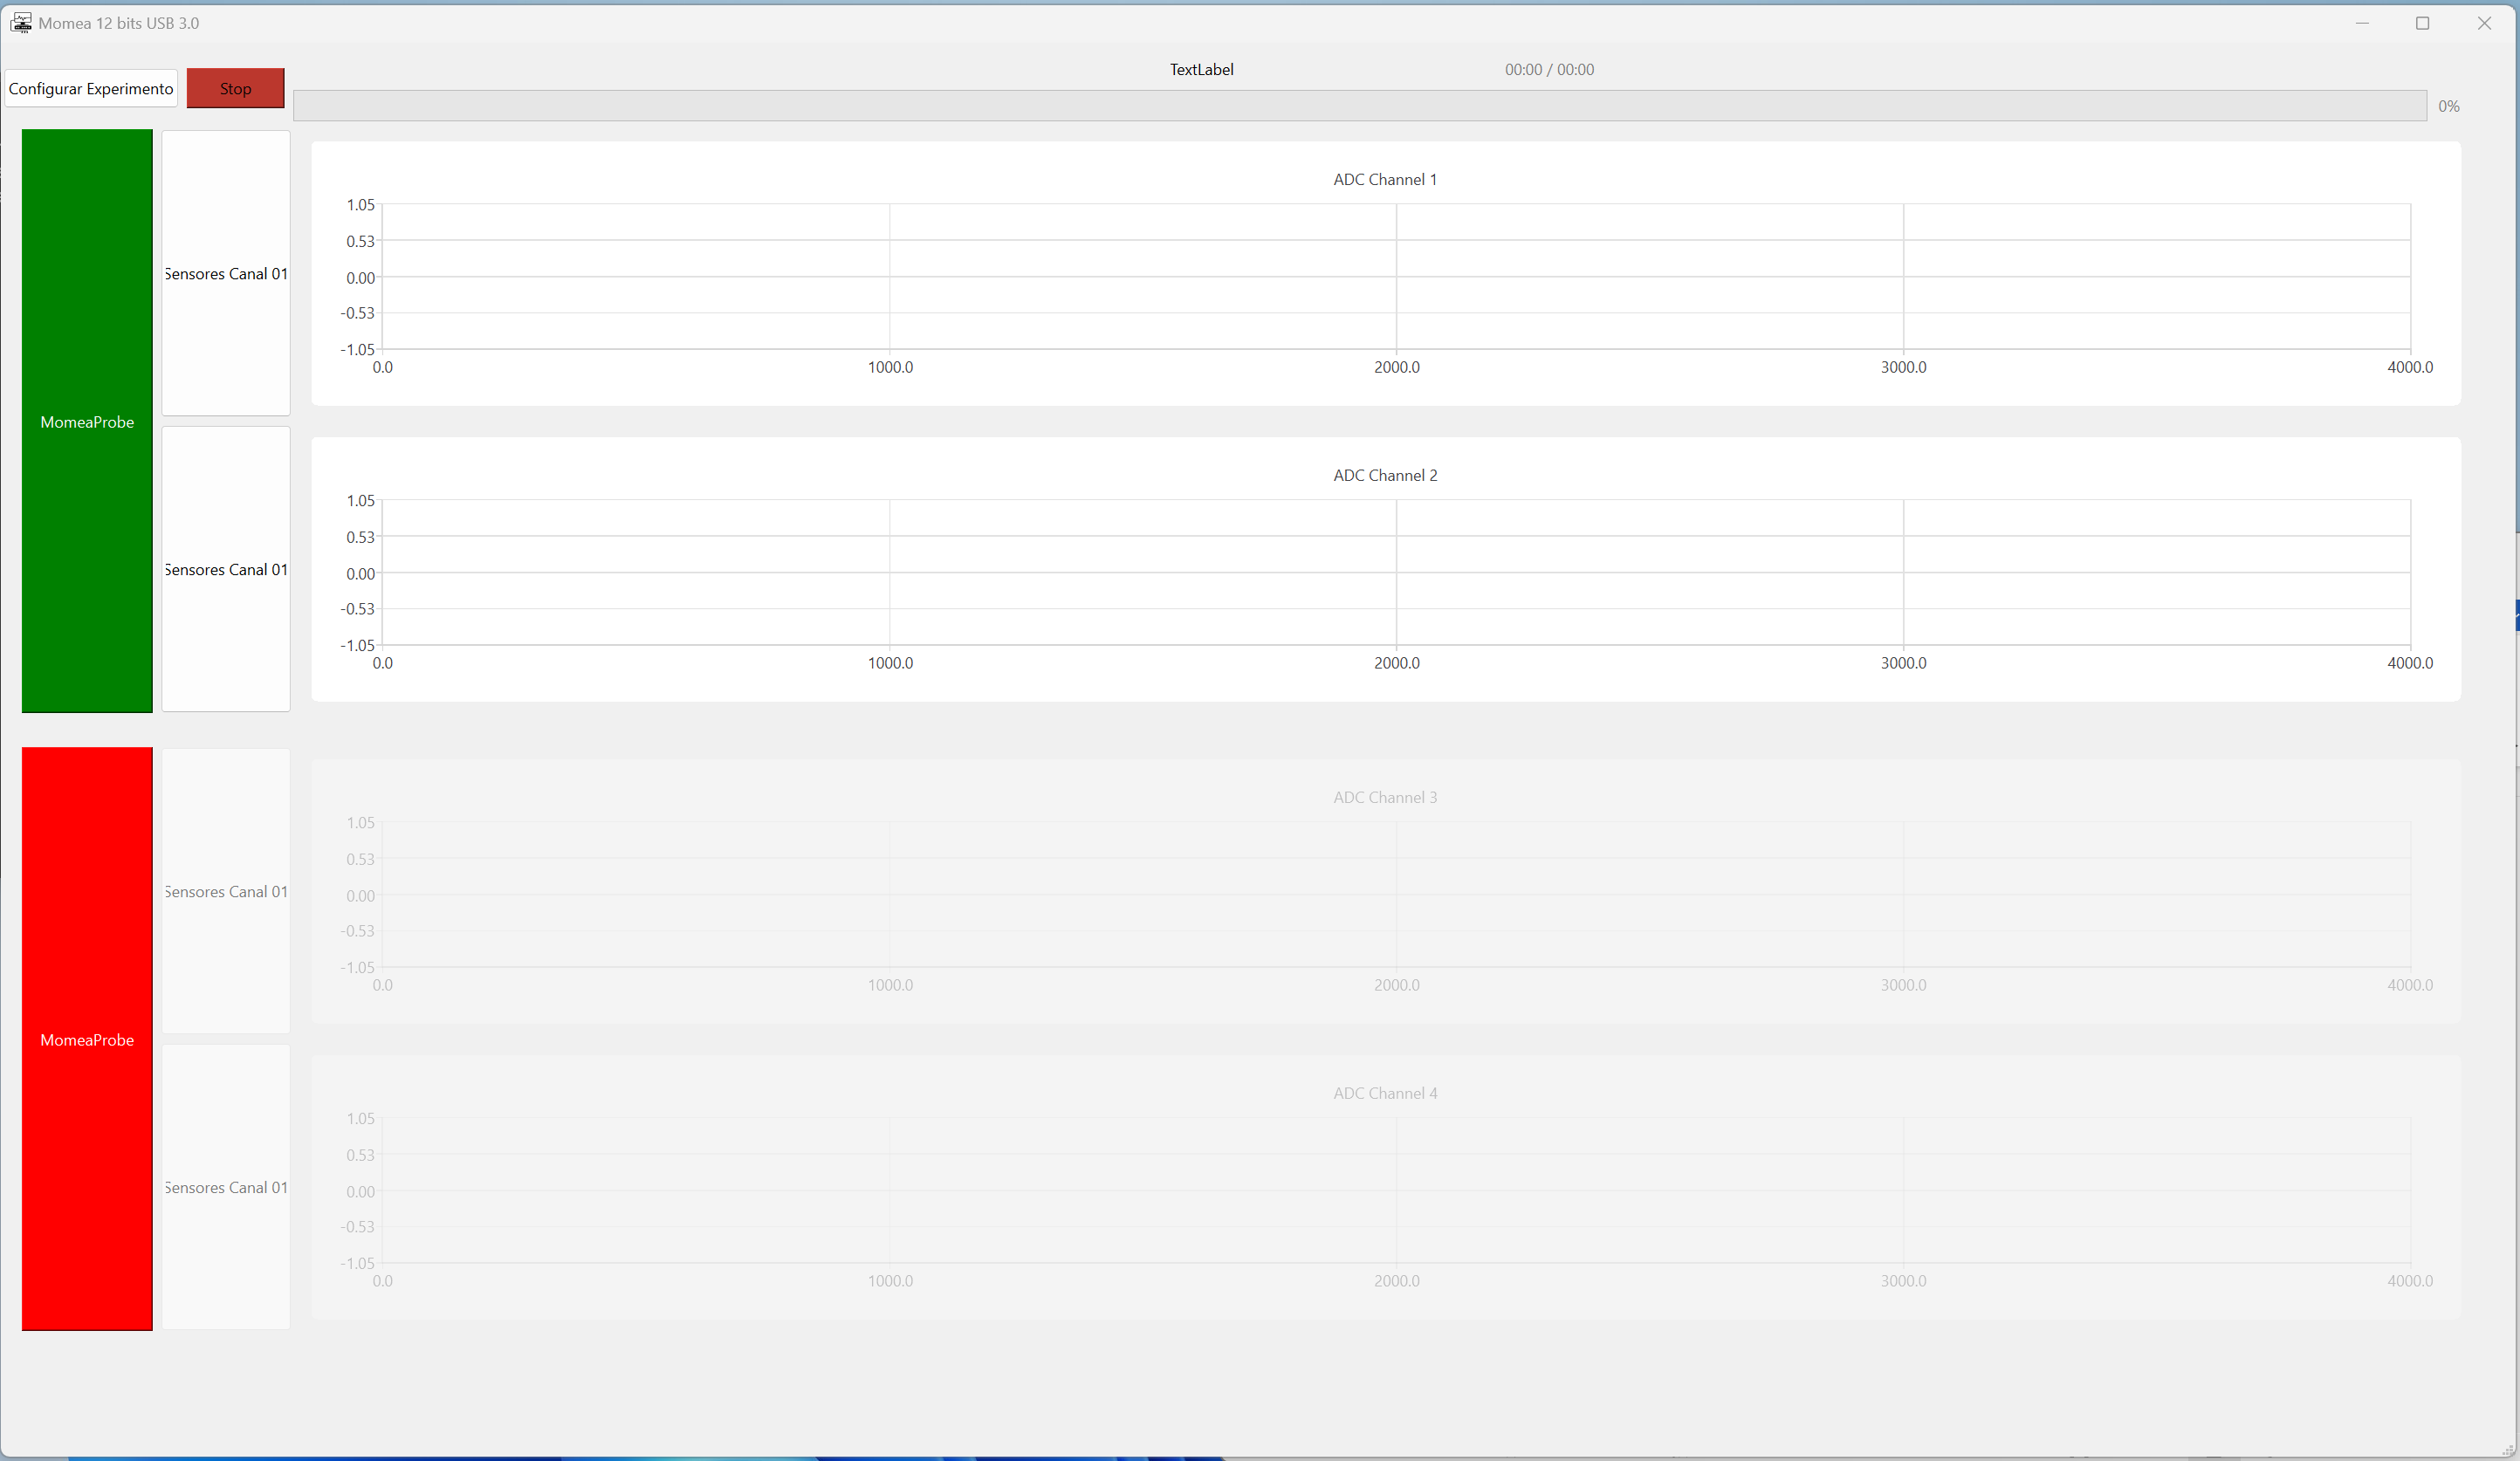
\includegraphics[width=0.5\linewidth]{figs/MomeaCapture.png}
    \caption{Software de captura MomeaCapture}
    \label{fig:MomeaCapture}
\end{figure}

Para a análise no domínio da frequência, foi implementado um módulo de processamento baseado na \textbf{Transformada Rápida de Fourier (FFT)} com janelamento móvel (\textit{short-time FFT}). Essa abordagem permite gerar imagens do espectro de frequência em função do tempo, produzindo mapas espectro-temporais semelhantes a espectrogramas. As imagens resultantes evidenciam o comportamento dinâmico dos componentes de alta frequência associados a eventos de cavitação, facilitando sua visualização e posterior interpretação automática.

A partir desses espectrogramas, foram treinadas redes neurais convolucionais bidimensionais (\textbf{CNN 2D}) — tradicionalmente empregadas em processamento de imagens — para identificar padrões característicos de cavitação em bombas centrífugas. O uso de CNNs 2D mostrou-se eficaz para distinguir condições normais, de cavitação incipiente e cavitação plenamente desenvolvida, aproveitando as propriedades espaciais e frequenciais extraídas das janelas espectrais.

Apesar dos resultados promissores, essa abordagem apresenta limitações inerentes ao grande volume de dados gerado e armazenado. O sistema MomeaProbe pode produzir dezenas de gigabytes por hora de operação contínua, o que é vantajoso durante a fase de treinamento dos modelos, mas inviável para o monitoramento em tempo real devido ao alto custo computacional e à latência de processamento. A geração de espectrogramas e a inferência em CNNs 2D exigem processamento intensivo, tornando o sistema dependente de GPU ou CPU de alto desempenho para alcançar taxas adequadas de atualização.

Diante dessas restrições, está em desenvolvimento uma solução baseada em \textbf{arquitetura FPGA-HIT (Hardware-in-the-Loop com Inferência Temporal)}, voltada à execução direta de inferência em tempo real no hardware reconfigurável. Essa nova abordagem, que será detalhada na próxima subseção, visa reduzir drasticamente a latência e o consumo de energia, mantendo a precisão do modelo por meio da quantização e otimização do pipeline de inferência embarcado.

\section{FPGA e Técnica de HIT}

Baseado na metodologia de detecção por \textbf{HIT (Hit Detection)}, descrita anteriormente na Seção~\ref{sec:UsoEA}, está em desenvolvimento uma implementação dedicada em \textbf{FPGA}, com o objetivo de realizar o pré-processamento e a filtragem dos sinais de Emissão Acústica (EA) diretamente no hardware, reduzindo significativamente o volume de dados a serem transmitidos e processados posteriormente no sistema de monitoramento.

A plataforma selecionada para essa implementação é a \textbf{Arty A7-35T}, da Digilent, mostrada na Figura \ref{fig:Arty} equipada com o \textbf{FPGA Xilinx Artix-7 XC7A35T}. Esse dispositivo conta com aproximadamente 33.280 células lógicas, 1.800~kB de memória interna distribuída (Block RAM), 90 blocos DSP~(Digital Signal Processing) e interfaces externas configuráveis. O Artix-7 oferece excelente equilíbrio entre custo, consumo energético e capacidade de processamento paralelo, sendo ideal para aplicações de prototipagem de sistemas embarcados de processamento em tempo real.

\begin{figure}[H]
    \centering
    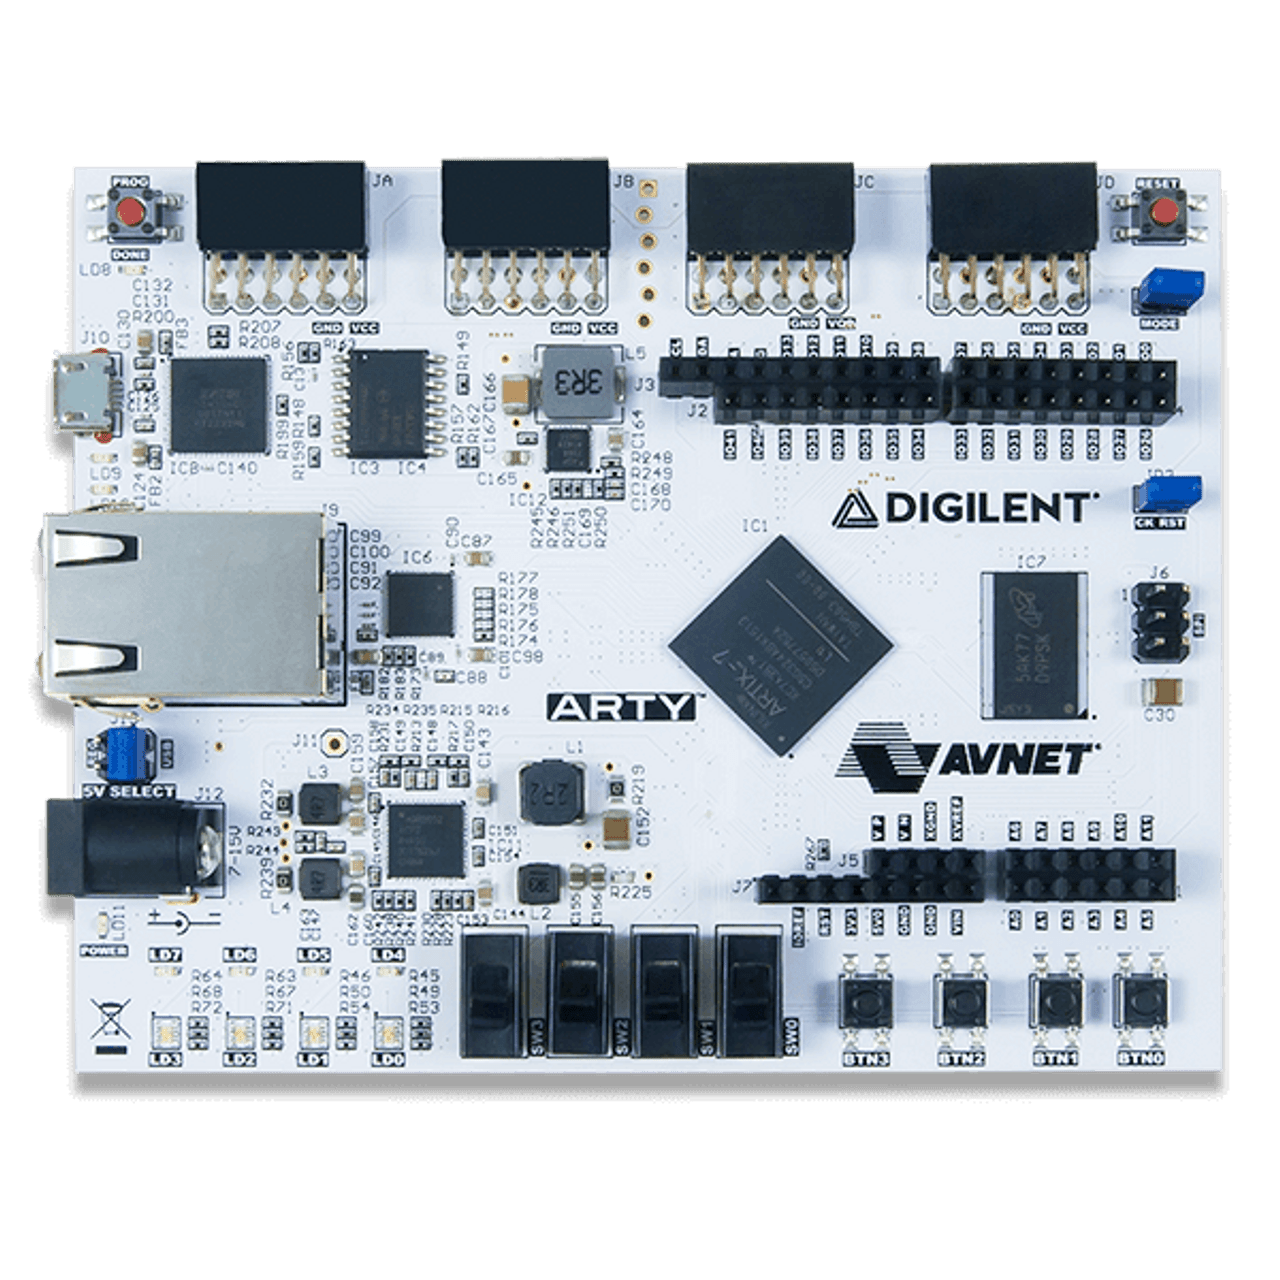
\includegraphics[width=0.5\linewidth]{figs/Arty_top.png}
    \caption{Placa de desenvolvimento Arty A7 35T.}
    \label{fig:Arty}
\end{figure}

Na arquitetura proposta, o FPGA executa o processamento de eventos de Emissão Acústica a partir da técnica de \textbf{detecção de HIT}, a qual identifica e caracteriza apenas os trechos do sinal que ultrapassam limiares definidos de amplitude ou energia. Esse método, conforme discutido na fundamentação teórica, permite registrar parâmetros essenciais de cada evento — como amplitude máxima, duração, energia e tempo de ocorrência — em vez de armazenar o sinal completo. Dessa forma, o volume de dados é reduzido em várias ordens de magnitude, o que viabiliza o monitoramento contínuo de longo prazo sem sobrecarregar a comunicação nem o armazenamento.

A implementação faz uso de uma \textbf{Soft CPU MicroBlaze}, processador configurável integrado ao FPGA e responsável pelo controle das tarefas de comunicação e gerenciamento do sistema. Sobre essa CPU, é executado o sistema operacional \textbf{FreeRTOS}, que permite o agendamento de múltiplas tarefas de forma determinística e de baixa latência, garantindo sincronismo entre a lógica de detecção de eventos e as rotinas de transmissão de dados.

A comunicação entre o módulo FPGA e o sistema de supervisão é realizada por meio de uma interface \textbf{Ethernet 10/100~Mbps}, implementada via controlador MAC interno e pilha TCP/IP embarcada. Esse canal é utilizado tanto para o envio dos eventos detectados quanto para o recebimento de comandos de configuração, como atualização de limiares, modos de operação e parâmetros de calibração.

Devido à natureza esparsa dos sinais de Emissão Acústica — em que longos períodos de silêncio são interrompidos por breves eventos de alta energia —, a técnica de HIT proporciona uma drástica redução no volume de dados transmitidos. Durante o regime normal de operação, em que não há eventos significativos, o tráfego de dados é mínimo. Mesmo durante a ocorrência de múltiplos eventos, a quantidade de informação permanece controlada, uma vez que apenas os descritores compactos de cada HIT são enviados.

Essa abordagem híbrida, combinando \textbf{processamento distribuído em hardware} e \textbf{controle multitarefa em software embarcado}, representa um avanço significativo rumo à \textbf{plataforma MOMEA-FPGA-HIT}, cuja meta é realizar a detecção de falhas em tempo real, com baixo consumo, alta confiabilidade e escalabilidade para integração em sistemas industriais. Os resultados preliminares indicam que essa arquitetura é capaz de reduzir substancialmente a latência de detecção e o volume de dados, mantendo a sensibilidade necessária para identificar fenômenos de cavitação e microtrincas em rotores de motobombas.

\subsection{Limitações do Método de HIT em Relação a Técnicas Baseadas em Aprendizado de Máquina}

Embora a técnica de detecção de eventos por \textbf{HIT} apresente vantagens significativas em termos de simplicidade, baixo custo computacional e eficiência no uso de memória, ela também possui limitações importantes quando comparada a abordagens baseadas em \textbf{aprendizado de máquina}, especialmente redes neurais convolucionais (\textit{Convolutional Neural Networks — CNNs}) e suas variantes unidimensionais (\textit{CNN-1D}).

A principal limitação do método de HIT reside no fato de que sua operação depende fortemente da definição de \textbf{limiares de detecção} (thresholds). Esses limiares são utilizados para identificar o instante em que a amplitude do sinal de Emissão Acústica (EA) ultrapassa um valor pré-determinado, indicando a ocorrência de um evento. No entanto, limiares mal ajustados podem levar a dois problemas críticos:

\begin{itemize}
    \item \textbf{Perda de eventos relevantes:}  
    Eventos de baixa amplitude — frequentemente associados a fenômenos incipientes, como o início da cavitação ou a formação de microtrincas — podem não ultrapassar o limiar definido e, portanto, não ser registrados. Essa limitação compromete a sensibilidade do sistema em detectar falhas em estágios iniciais.

    \item \textbf{Falsos negativos e dependência de calibração:}  
    O desempenho do método depende fortemente da calibração experimental, que pode variar conforme o tipo de sensor, o acoplamento mecânico, o ruído estrutural e as condições de operação da máquina. Pequenas variações nessas condições podem alterar significativamente a amplitude dos sinais, exigindo reconfigurações frequentes dos parâmetros de detecção.
\end{itemize}

Além disso, o método de HIT não considera a \textbf{estrutura temporal e espectral completa} do sinal, pois registra apenas parâmetros estatísticos resumidos — como amplitude máxima, duração, energia e número de contagens — sem preservar a forma de onda original. Isso limita a capacidade do sistema de capturar padrões complexos ou sutis que poderiam ser indicativos de processos físicos distintos, como cavitação transitória, impactos mecânicos ou ruídos estruturais.

Em contraste, modelos de aprendizado profundo, como as \textbf{CNNs 2D} e \textbf{CNN-1D}, analisam diretamente os sinais brutos ou suas representações espectro-temporais, aprendendo automaticamente características discriminativas que podem não ser evidentes a partir de parâmetros manuais. Essas redes são capazes de detectar relações não lineares, correlações temporais e variações espectrais de pequena magnitude, o que as torna particularmente eficazes para identificar estágios iniciais de cavitação ou falhas de natureza intermitente.

Por fim, embora o método de HIT seja extremamente eficiente para \textbf{monitoramento contínuo embarcado}, ele se mostra limitado em cenários que demandam \textbf{diagnóstico detalhado ou classificação precisa de eventos}. Assim, uma solução híbrida — na qual a detecção inicial por HIT seja complementada por um módulo de inferência baseado em CNN embarcado em FPGA — surge como uma alternativa promissora, combinando a eficiência do pré-processamento em hardware com o poder discriminativo do aprendizado profundo.

\section{Resultados Parciais e Proposta de Pesquisa}

Os resultados obtidos até o momento demonstram a viabilidade da detecção de cavitação em bombas centrífugas por meio da análise espectro-temporal de sinais acústicos, utilizando redes neurais convolucionais (\textbf{CNNs}) aplicadas a imagens de espectrogramas geradas a partir da Transformada Rápida de Fourier (FFT) janelada. Essa abordagem, implementada no ambiente de software \textbf{MomeaCapture}, tem se mostrado eficaz para classificar diferentes estágios de cavitação e distinguir condições de operação normais, incipientes e severas. No entanto, sua principal limitação reside no elevado volume de dados processados e na latência associada ao fluxo contínuo de aquisição via USB~3.0, o que restringe sua aplicação em monitoramento em tempo real.

Para superar essas limitações, propõe-se o estudo e a simulação de uma arquitetura embarcada de \textbf{inferência em FPGA}, baseada em uma rede \textbf{CNN-1D} otimizada e quantizada. Essa proposta busca unir o poder discriminativo das redes neurais convolucionais — capazes de identificar padrões sutis e não lineares mesmo em sinais compactados — com a eficiência e o paralelismo inerentes ao hardware reconfigurável. O objetivo é possibilitar o \textbf{processamento em tempo quase real} (\textit{near real-time}) diretamente no dispositivo, reduzindo significativamente a latência e o volume de dados transmitidos, de modo que apenas alertas de falhas ou eventos relevantes sejam enviados ao sistema de monitoramento superior.

% A comparação entre as duas abordagens pode ser sintetizada da seguinte forma:

% \begin{table}[H]
% \centering
% \caption{Comparação entre os métodos contínuo (USB + CNN 2D) e embarcado (FPGA + HIT + CNN 1D).}
% \label{tab:comparacao_usb_fpga}
% \renewcommand{\arraystretch}{1.3}
% \resizebox{\textwidth}{!}{
% \begin{tabular}{p{4.2cm} p{5.3cm} p{5.3cm}}
% \hline
% \textbf{Aspecto} & \textbf{Método Contínuo (USB + CNN 2D)} & \textbf{Método Embarcado (FPGA + HIT + CNN 1D)} \\ \hline
% \textbf{Aquisição de Dados} & Fluxo contínuo via USB~3.0 (40~Msps por canal) & Aquisição seletiva por eventos (HITs) via ADC interno \\ \hline
% \textbf{Pré-processamento} & FFT janelada e geração de espectrogramas & Detecção de HIT e extração de parâmetros compactos \\ \hline
% \textbf{Modelo de IA} & CNN 2D aplicada a imagens espectro-temporais & CNN 1D aplicada a trechos de sinal compactado \\ \hline
% \textbf{Volume de Dados} & Elevado — dezenas de GB/hora & Reduzido — apenas eventos relevantes \\ \hline
% \textbf{Latência de Processamento} & Alta — dependente de GPU/CPU & Baixa — inferência em hardware dedicada \\ \hline
% \textbf{Consumo de Energia} & Alto (processamento contínuo) & Baixo (ativação sob demanda) \\ \hline
% \textbf{Aplicação Ideal} & Treinamento e análise off-line & Monitoramento contínuo embarcado em campo \\ \hline
% \end{tabular}}
% \end{table}

% Com base nesses resultados e na análise comparativa apresentada, o desenvolvimento do sistema \textbf{FPGA + HIT + CNN-1D} representa o próximo passo natural do projeto MOMEA. Essa solução busca aliar a precisão do aprendizado profundo à eficiência da computação reconfigurável, estabelecendo as bases para uma plataforma de \textbf{monitoramento inteligente em tempo real} capaz de detectar cavitação e falhas incipientes com alta sensibilidade e confiabilidade, diretamente no ambiente industrial.
